\section{ Thermal cameras}

Thermal cameras are transducers that convert infrared (IR) radiation into electrical signals, which can be used to form a thermal image.
IR is an electromagnetic (EM) radiation and covers part of EM spectrum that is invisible to the human eye.
IR spectrum covers wavelengths from 780 \si{\micro\meter} to 1 \si{\milli\meter}, but only small part of that spectrum is used for IR imaging ( from 0.9 \si{\micro\meter} to 14 \si{\micro\meter})\cite{thermal_book}.
We can broadly classify IR cameras into two categories: photon detectors or thermal detectors\cite{thermal_book}.
Photon detectors convert absorbed EM radiation directly into electric signals by the change of concentration of free charge carriers\cite{thermal_book}.
Thermal detectors covert absorbed EM radiation into thermal energy, raising the detector temperature\cite{thermal_book}. 
Change of detector's temperature is then converted into an electrical signal.
Since photon detectors are expensive, large and therefore unsuitable for our use case, we will not describe them in greater detail.

Common examples of thermal detectors are thermopiles and microbolometers. 
Thermopiles are composed of several thermocouples.
Thermocouples consists of two different metals joined at one end, which is known as hot junction.
Other two ends of the metals are known as cold junctions.
When there is a temperature difference between the hot and cold junctions, voltage proportional to that difference is generated on open ends of the metals.
To increase voltage responsivity, several thermocouples are connected in series to form a thermopile\cite{thermal_book}.
Thermopiles have lower responsivity when compared to microbolometers, but they do not require temperature stabilization\cite{thermal_book}.

Microbolometers can be found in most IR cameras today\cite{thermal_book}. 
They are sensitive to IR wavelengths of 8 to 14 \si{\micro\meter}, which is a part of longwave infrared region (LWIR)\cite{thermal_book}.
Measuring part of an microbolometer is known as focal point array (FPA) (Figure \ref{FPA}).
FPA consists of IR thermal detectors, bolometers (Figure \ref{FPA_pixel}), that convert IR radiation into electric signal.
Each bolometer consists of an absorber material connected to an readout integrated circuit (ROIC) over thermally insulated, but electrically conductive legs\cite{thermal_article}.
\newline

\begin{figure}[h]
    \begin{subfigure}{0.5\textwidth}
        \centering
        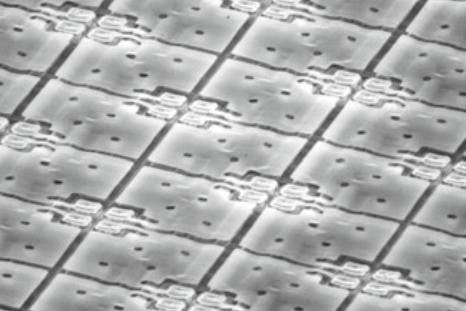
\includegraphics[width=1.0\linewidth, height=5cm]{FPA.png} 
        \caption{}
        \label{FPA}
    \end{subfigure}
    \begin{subfigure}{0.5\textwidth}
        \centering
        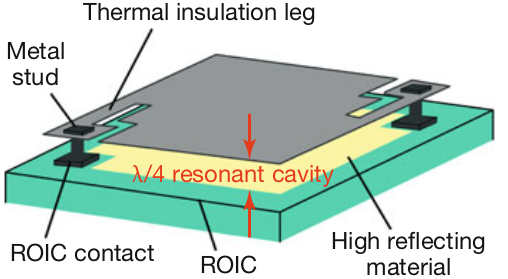
\includegraphics[width=1.0\linewidth, height=5cm]{FPA_pixel.png}
        \caption{}
        \label{FPA_pixel}
    \end{subfigure}

    \caption{(a) Focal point array under electronic microscope. (b) Bolometer with $\lambda /4$ resonant cavity. Image source: Vollmer, Möllmann\cite{thermal_book}}
    \label{FPA_microbolo}
\end{figure}

Absorber material is made either out of metals such as gold, platinum, titanium or more commonly out of semiconductors such as vanadium-oxide (VOx)\cite{thermal_article}.
Important property of absorber materials is that electrical resistance changes proportionally with material's temperature\cite{thermal_book}.
When IR radiation hits absorber material, it is converted into thermal energy, which raises absorber's temperature, thus changing its resistance.
To detect change in resistance, ROIC applies steady-state bias current to absorber material, while measuring voltage over conductive legs\cite{thermal_book}. 

When deciding between different types of thermal cameras we are often comparing them in the terms of cost, size and image resolution.
One important property that also has to be taken into account is temperature sensitivity, also known as noise equivalent temperature difference (NETD).
NETD is measured in \si{\milli\kelvin} and tells us minimum temperature difference that can still be detected by a thermal camera.
In microbolometers NETD is proportional to the thermal conductance of absorber material, among other factors\cite{thermal_book}.
Thermal conductance of bolometers is minimized by enclosing FPA into vacuum chamber, thus excluding thermal convection and conduction due to surrounding gasses.
Only means of heat transfer that remain are radiant heat exchange (highly reflective material below absorber is minimizing its radiative losses) and conductive heat exchange through supportive legs.
NETD also depends on the temperature inside the camera, higher ambient temperatures can raise the internal temperature, thus increasing NETD and noise present in thermal image.
Today's thermopiles can achieve NETD of 100 \si{\milli\kelvin}, microbolometers 45 \si{\milli\kelvin}, while photon detectors can have NETD of 10 \si{\milli\kelvin}.
Although tens of \si{\milli\kelvin} does not seem a lot, we can see on Figure \ref{NETD} what a difference of 20 \si{\milli\kelvin} means for image resolution and noise.
\newline

\begin{figure}[h]
    \begin{subfigure}{0.5\textwidth}
        \centering
        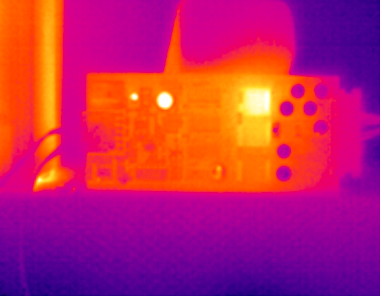
\includegraphics[width=1.0\linewidth, height=5cm]{NETD_60mk.png} 
        \caption{NETD is 60 \si{\milli\kelvin}}
        \label{NETD_60mk}
    \end{subfigure}
    \begin{subfigure}{0.5\textwidth}
        \centering
        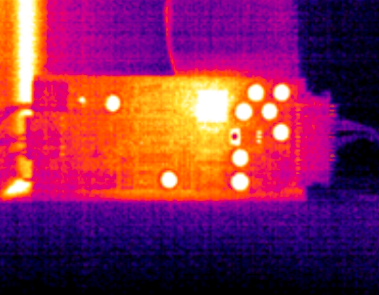
\includegraphics[width=1.0\linewidth, height=5cm]{NETD_80mk.png}
        \caption{NETD is 80 \si{\milli\kelvin}}
        \label{NETD_80mk}
    \end{subfigure}

    \caption{Comparison of images of the same object taken with cameras with different NETD values. Low NETD values are more appropriate for object recognition. Image source: MoviTherm \cite{NETD}}
    \label{NETD}
\end{figure}


\subsection{ Choosing the thermal camera}

Choice of thermal camera was made by Arribada Initiative\cite{thermal_comparison}.
They tested several different thermopiles and microbolometers, while searching for desired properties.
Camera had to be relatively inexpensive and small enough so that it could be integrated into relatively small housing.
Main property that they searched for was that elephants could be easily recognized from thermal images.
That meant that camera needed to have decent resolution and low NETD.
Cameras were tested in Whipsnade Zoo and the Yorkshire Wildlife Park where images of elephants and polar bears could be made.

They tested two thermopile cameras (Heimann 80x64, MELEXIS MLX90640) and two microbolometer cameras (ULIS Micro80 Gen2, FLIR Lepton 2.5).
Although thermopile cameras were cheaper from microbolometer cameras, quality of images they produced was inferior, as can be seen on Figure \ref{thermal_comparison_images}
MELEXIS MLX90640 camera had resolution of 32 x 24 pixels and NETD of 100 \si{\milli\kelvin}, while Heimann camera had resolution of 80 x 64 pixels and NETD of 400 \si{\milli\kelvin}.
\newline

\begin{figure}[h]
    \begin{subfigure}{0.5\textwidth}
        \centering
        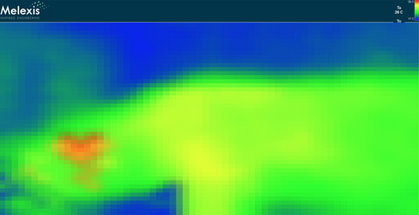
\includegraphics[width=1.0\linewidth, height=5cm]{thermal_comparison_a.png} 
        \label{thermal_comparison_a}
    \end{subfigure}
    \begin{subfigure}{0.5\textwidth}
        \centering
        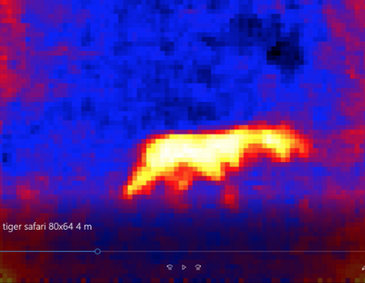
\includegraphics[width=1.0\linewidth, height=5cm]{thermal_comparison_b.png} 
        \label{thermal_comparison_b}
    \end{subfigure}
    \begin{subfigure}{0.5\textwidth}
        \centering
        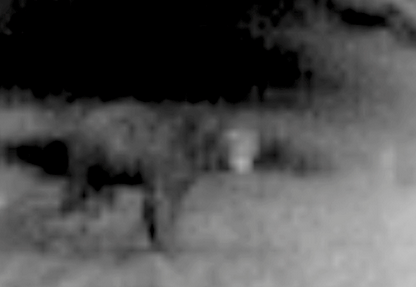
\includegraphics[width=1.0\linewidth, height=5cm]{thermal_comparison_c.png} 
        \label{thermal_comparison_c}
    \end{subfigure}
    \begin{subfigure}{0.5\textwidth}
        \centering
        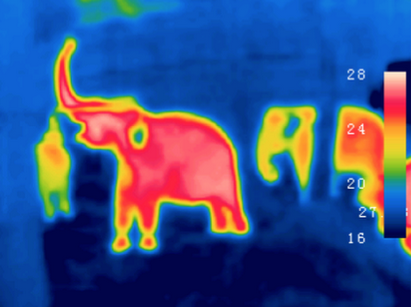
\includegraphics[width=1.0\linewidth, height=5cm]{thermal_comparison_d.png} 
        \label{thermal_comparison_d}
    \end{subfigure}

\caption{Comparison of image quality made by different thermal cameras, MELEXIS MLX90640 (top left), Heimann 80x64 (top right), ULIS Micro80 Gen2 (bottom left) and FLIR Lepton 2.5 (bottom right). Image source: Arribada Initiative \cite{thermal_comparison}}
    \label{thermal_comparison_images}
\end{figure}

It was concluded that images taken by either one of thermopile cameras could not be used for object recognition, merely only if object was present or not\cite{thermal_comparison}.

Microbolometers produced better results.
Both Ulis Micro80 and FLIR Lepton had similar resolution, 80 x 80 and 80 x 60 respectively, but Ulis Micro80 had two times bigger NETD compared to FLIR Lepton camera, 100 \si{\milli\kelvin} and 50 \si{\milli\kelvin}, respectively.
Images produced by FLIR Lepton were much cleaner, so it was chosen as appropriate camera for the task.

It is important to note that FLIR Lepton, as all microbolometers, requires frequent calibration to function properly.
In temperature non-stabilized cameras small temperature drifts can have a major impact on image quality\cite{thermal_book}.
Calibration is done either by internal algorithms of the camera or by exposing the camera to uniform thermal scene.
FLIR Lepton camera comes with a shutter, which acts as a uniform thermal signal and enables regular calibration.
Calibration in FLIR Lepton is by default automatic, triggering at startup and every 3 minutes afterwards or if camera temperature drifts for more than 1.5 \si{\celsius}.


    2.2 Wireless technologies in IOT world
        different technologies, tradeoffs, why do we want lora. 
        2.2.2 LoRa 
            How does it work, what is the ecosystem around it, power consumption, data transmission (compare with some other things) 
    2.3 Neural networks
        What neural networks are, what is their point, forward propagation, back propagation, what kinds of neural networks exist, which ones are interesting for me.
    2.4 TensorFlow
        Describe the framework, what are alternatives, how does it work for you (meaning what programmer doesn't need to care about).
        2.4.1 TensorFlow Lite for microcontollers
            What this is, how is given to developers, describe generic flow from a model to deploying it.
    2.5 Solar panels
        How they work, types, expected power output
    2.6 Battery technologies
        Princips of operation, types, focus on the one you will use, Lipo 
    Above two chapters should be short.

